% TEMPLATE.TEX
%
% Time-stamp: <2013-03-26 11:09 olenz>
%
% This is an extensively documented LaTeX file that shows how to
% produce a good-looking document with current LaTeX (11/2012).
%
% IMPORTANT!
%
%   Some obsolete commands and packages
% ----------|-------------------------------
% obsolete  |     Replacement in LATEX 2ε
% ----------|-------------------------------
%           | local            global/switch
% ----------|-------------------------------
% {\bf ...} | \textbf{...}     \bfseries
%     -     | \emph{...}       \em
% {\it ...} | \textit{...}     \itshape
%     -     | \textmd{...}     \mdseries
% {\rm ...} | \textrm{...}     \rmfamily
% {\sc ...} | \textsc{...}     \scshape
% {\sf ...} | \textsf{...}     \sffamily
% {\sl ...} | \textsl{...}     \slshape
% {\tt ...} | \texttt{...}     \ttfamily
%     -     | \textup{...}     \upshape
%
% DON'T USE \\ TO MAKE LINEBREAKS, INSTEAD JUST LEAVE A BLANK LINE!
%
\RequirePackage[l2tabu,orthodox]{nag} % turn on warnings because of bad style
\documentclass[a4paper,10pt,bibtotoc]{scrartcl}
%
\usepackage[bottom=3.5cm, top=2cm]{geometry}
%%%%%%%%%%%%%%%%%%%%%%%%%%%%%%%%%%%%
% KOMA CLASSES
%%%%%%%%%%%%%%%%%%%%%%%%%%%%%%%%%%%%
%
% The class "scrartcl" is one of the so-called KOMA-classes, a set of
% very well done LaTeX-classes that produce a very European layout
% (e.g. titles with a sans-serif font).
%
% The KOMA classes have extensive documentation that you can access
% via the commands:
%   texdoc scrguide # in German
%   texdoc scrguien # in English
%
%
% The available classes are:
%
% scrartcl - for "articles", typically for up to ~20 pages, the
%            highest level sectioning command is \section
%
% scrreprt - for "reports", typically for up to ~200 pages, the
%            highest level sectioning command is \chapter
%
% scrbook  - for "books", for more than 200 pages, the highest level
%            sectioning command is \part.
%
% USEFUL OPTIONS
%
% a4paper  - Use a4 paper instead of the default american letter
%            format.
%
% 11pt, 12pt, 10pt
%          - Use a font with the given size.
%
% bibtotoc - Add the bibliography to the table of contents
%
% The KOMA-script classes have plenty of options to modify

% This allows to type UTF-8 characters like ä,ö,ü,ß
\usepackage[utf8]{inputenc}

\usepackage[T1]{fontenc}        % Tries to use Postscript Type 1 Fonts for better rendering
\usepackage{lmodern}            % Provides the Latin Modern Font which offers more glyphs than the default Computer Modern
\usepackage[intlimits]{amsmath} % Provides all mathematical commands

\usepackage{hyperref}           % Provides clickable links in the PDF-document for \ref
\usepackage{graphicx}            % Allow you to include images (like graphicx). Usage: \includegraphics{path/to/file}

% Allows to set units
\usepackage[ugly]{units}        % Allows you to type units with correct spacing and font style. Usage: $\unit[100]{m}$ or $\unitfrac[100]{m}{s}$

% Additional packages
\usepackage{url}                % Lets you typeset urls. Usage: \url{http://...}
\usepackage{breakurl}           % Enables linebreaks for urls
\usepackage{xspace}             % Use \xpsace in macros to automatically insert space based on context. Usage: \newcommand{\es}{ESPResSo\xspace}
\usepackage{xcolor}             % Obviously colors. Usage: \color{red} Red text
\usepackage{booktabs}           % Nice rules for tables. Usage \begin{tabular}\toprule ... \midrule ... \bottomrule

% Source code listings
\usepackage{listings}           % Source Code Listings. Usage: \begin{lstlisting}...\end{lstlisting}
\lstloadlanguages{python}
\definecolor{lightpurple}{rgb}{0.8,0.8,1}

\lstset{
stepnumber=1,
numbersep=5pt,
numberstyle=\small\color{black},
basicstyle=\ttfamily,
%keywordstyle=\color{black},
%commentstyle=\color{black},
%stringstyle=\color{black},
frame=single,
tabsize=4,
language = python,
backgroundcolor=\color{black!5}}

\usepackage{float}

\begin{document}

\titlehead{Simulation Methods in Physics II \hfill SS 2020}
\title{Report for Worksheet 1: Calculate solid crystalline materials using density functional theory}
\author{Markus Baur and David Beyer}
\date{\today}
\maketitle

\tableofcontents

\section{Short Questions --Short Answers}
\begin{itemize}
 \item \textbf{A1}: Density functional theory is computationally more efficient than Hartree-Fock. For this reason, it is often useful to use DFT to investigate system which have many electrons, like crystals in solid state physics or big molecules.
 
\item \textbf{A2}: Because the energy density functional of a given system is minimized by the electron density of the ground state (Hohenberg-Kohn theorem II), we can also obtain the ground state energy by describing a given system as a system of non-interacting particles in an effective potential with the same electron density. 
The one-particle differential equations for these ficitious particles are obtained by minimizing the energy functional and are known as Kohn-Sham equations. 
The Kohn-Sham equations have the form of one-particle Schrödinger equations with the difference that the effective potential depends on the electron density.
The effective potential appearing in the Kohn-Sham equations contains the external potential, electron repulsion and a term accounting for the exchange correlation.
 
 \item \textbf{A3}: LDA stands for local density approximation. In the LDA, the exchange-correlation energy is a local functional of the electron density $n\left(\mathbf{r}\right)$, this means that it only depends on the value at each point separately. 
 We can thus write it as an integral which contains no derivatives of the density. 
 GGA stands for generalized gradient approximation, as the name suggest, the energy functional not only depends on the electron density but also on its derivatives. 
 This means that in contrast to LDA the exchange-correlation energy for GGA is not a local, but a semilocal functional of the electron density.

 \item \textbf{A4}: The van-der-Waals interaction is effectively caused by longe-range correlations of the electrons.
 Because LDA and GGA are (semi-)local approximations to the exchange correlation energy functional, they cannot account for this non-local effect.
 
 \item \textbf{A5}: Because we don't know the exact exchange correlation energy functional, we have to use approximations like LDA or GGA. 
 These (semi-)local approximations cause the so-called self-interaction error: the effective potential appearing in the Kohn-Sham equations depends on electron density, this means that every fictious electron will also interact with itself through its own density.
\end{itemize}


\section{Quantum Mechanical Calculations using CP2K}
The following section deals with DFT-calculations for diamond.

\subsection{Converging the Cutoff Energy}
In order to find an appropriate cutoff energy, we ran calculations with different values of the cutoff energy (between 50 and 450 Rydberg). REL\_CUTOFF was set to 60 Rydberg. \autoref{fig:fig1} shows the computed total energies as a function of the cutoff energy. We can clearly see that the total energy sharply decreases when the cutoff energy is increased from 50 Ry to 100 Ry. However, a further increase in the cutoff energy does not change much. Because of this, we used a cutoff energy of 100 Ry in the following simulations.

\begin{figure}[h]
\centering
 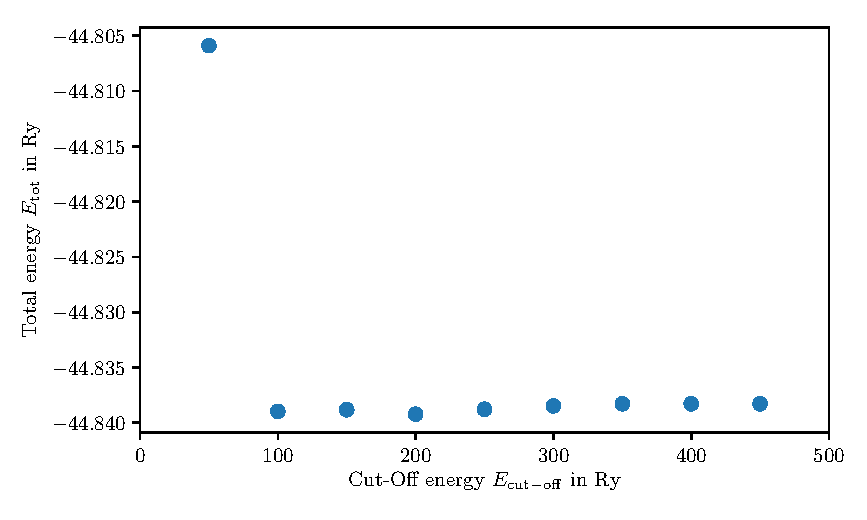
\includegraphics[width=\textwidth]{Figure_cutoff_energy.pdf}
 \caption{Plot of the calculated total energy for different cutoff energies.}
 \label{fig:fig1}
\end{figure}

\subsection{Optimzing the Lattice Constant}
To optimize the crystal structure, we ran calculations with the RUN\_TYPE GEO\_OPT and different values of the lattice constant. We could then determine the equilibirium lattice constant using a fit.

\subsubsection{PBE Functional}
\autoref{fig:fig2} shows the calculated total energy as a function of the volume $V=a^3$ of the unit cell. It is easy to see that there is a minimum. In order to determine the corresponding equilibrium volume, we fitted the quadratic function
\begin{align}
f(V) = a + b\cdot\left(V-V_\mathrm{eq}\right)^2
\end{align}
to the calculated values, this is also shown in the plot. The obtained fit parameters are
\begin{align}
a &= -44.9809763\,\mathrm{Ry}\\
b &= 7.72048911\cdot 10^{-4}\,\frac{\mathrm{Ry}}{\r{A}^6}\\
V_\mathrm{eq} &= 50.7015415\,\r{A}^3.
\end{align}
The equilibrium lattice constant can be calculated from $V_\mathrm{eq}$ and is given by
\begin{align}
a_\mathrm{eq} = \sqrt[3]{V_\mathrm{eq}} \approx 3.70\,\r{A}.
\end{align}
This value is about 3\% larger than the experimental value of $a_\mathrm{eq,exp.} \approx 3.57\,\r{A}$\footnote{http://lampx.tugraz.at/~hadley/ss1/crystalstructure/structures/diamond/diamond.php, accessed on April 30, 2020 at 22:00}, which means that PBE overestimates the lattice constant.
PBE is a GGA functional which is known to overestimate lattice constants.

\autoref{fig:fig3} shows a visualization of the primitive unit cell of diamond which was created using the software VMD (Visual Molecular Dynamics). The structure was taken from the simulation with the equilibrium lattice constant determined above.


\begin{figure}[h]
\centering
 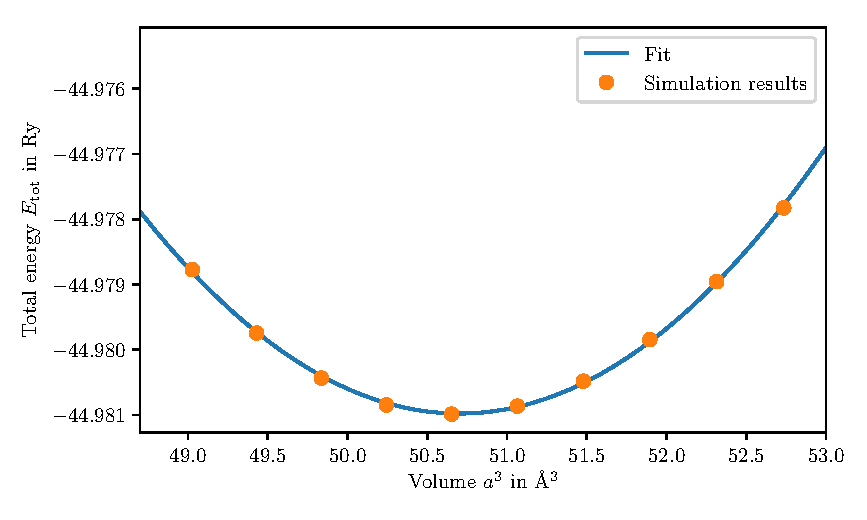
\includegraphics[width=\textwidth]{Figure_lattice_constant_PBE.pdf}
 \caption{Plot of the calculated total energy (using the PBE functional) as a function of the volume of the unit cell. The fit-function which is also shown is a parabola which was fitted to the obtained values in order to determine the equilibrium lattice constant.}
 \label{fig:fig2}
\end{figure}

\begin{figure}[h]
\centering
 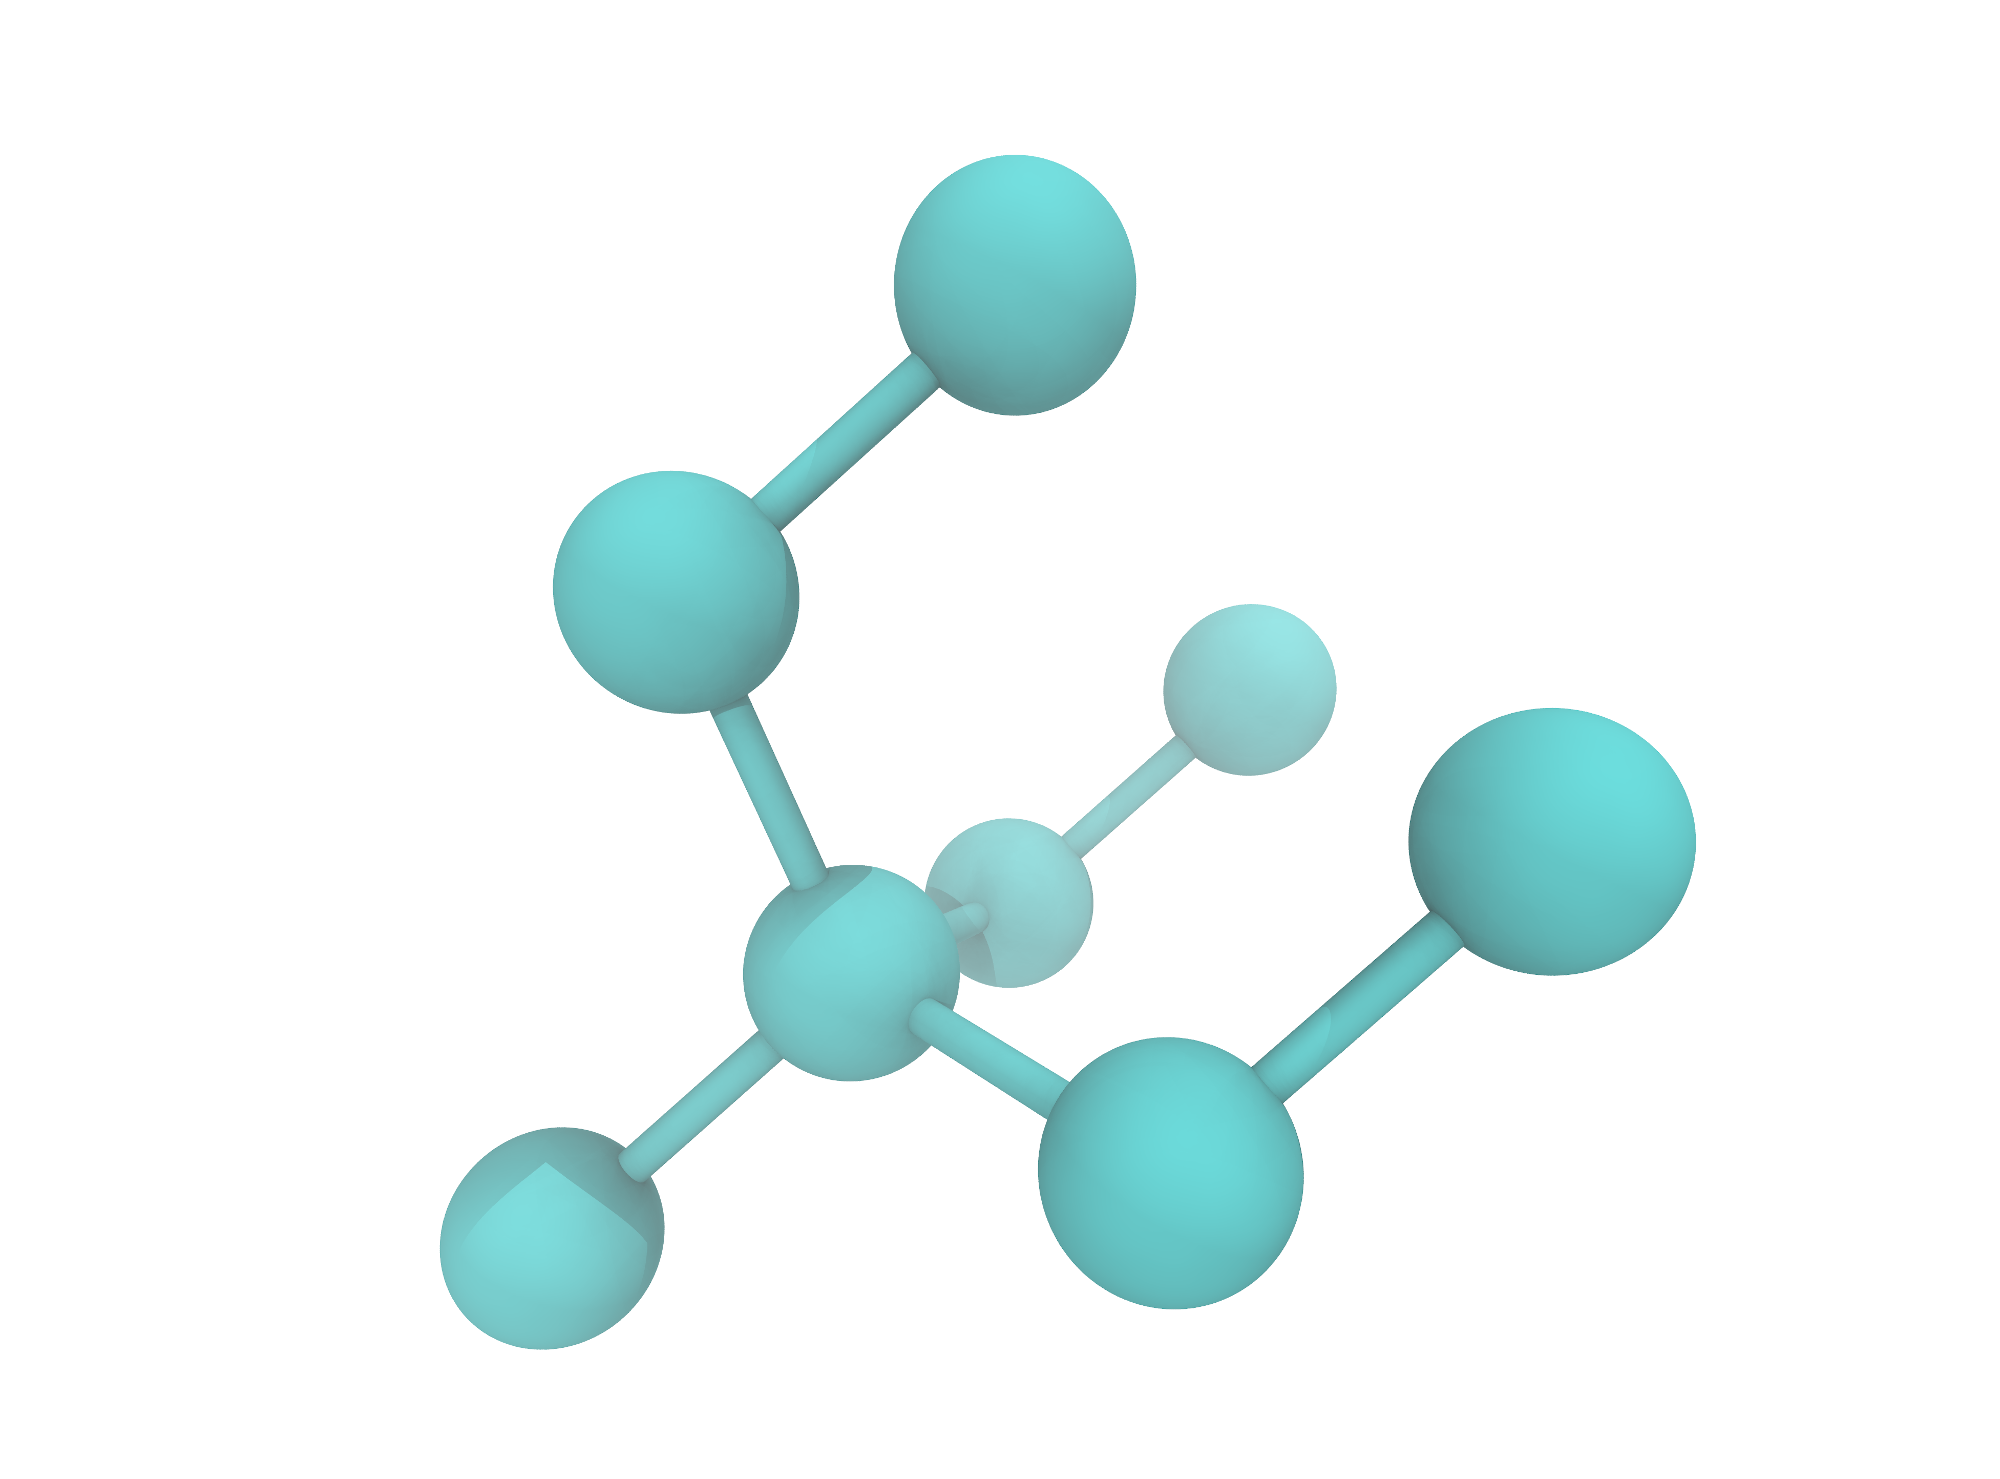
\includegraphics[width=\textwidth]{structure.png}
 \caption{Visualization of the crystal structure of diamond. The shown selection corresponds to the primite unit cell.}
 \label{fig:fig3}
\end{figure}

\subsubsection{LDA Functional}
In order to use the LDA functional we have to change the input at two places /the exchange correlation functional and the potential):
\begin{lstlisting}
&XC
    &XC_FUNCTIONAL LDA
    &END XC_FUNCTIONAL
&END XC
\end{lstlisting}
\begin{lstlisting}
&KIND C
    POTENTIAL GTH-PADE-q4
    BASIS_SET DZVP-MOLOPT-SR-GTH
&END KIND
\end{lstlisting}



\autoref{fig:fig2x} shows the calculated total energy as a function of the volume $V=a^3$ of the unit cell. It is easy to see that there is a minimum. In order to determine the corresponding equilibrium volume, we fitted the quadratic function
\begin{align}
f(V) = a + b\cdot\left(V-V_\mathrm{eq}\right)^2
\end{align}
to the calculated values, this is also shown in the plot. The obtained fit parameters are
\begin{align}
a &= -45.1151414\,\mathrm{Ry}\\
b &= 1.01386118\cdot 10^{-3}\,\frac{\mathrm{Ry}}{\r{A}^6}\\
V_\mathrm{eq} &= 48.4645445\,\r{A}^3.
\end{align}
The equilibrium lattice constant can be calculated from $V_\mathrm{eq}$ and is given by
\begin{align}
a_\mathrm{eq} = \sqrt[3]{V_\mathrm{eq}} \approx 3.65\,\r{A}.
\end{align}
This value is about 2\% larger than the experimental value of $a_\mathrm{eq,exp.} \approx 3.57\,\r{A}$\footnote{http://lampx.tugraz.at/~hadley/ss1/crystalstructure/structures/diamond/diamond.php, accessed on April 30, 2020 at 22:00} but smaller than the value which was obtained using PBE. This is rather unexpected since LDA methods normally tend to underestimate lattice constants.

\begin{figure}[h]
\centering
 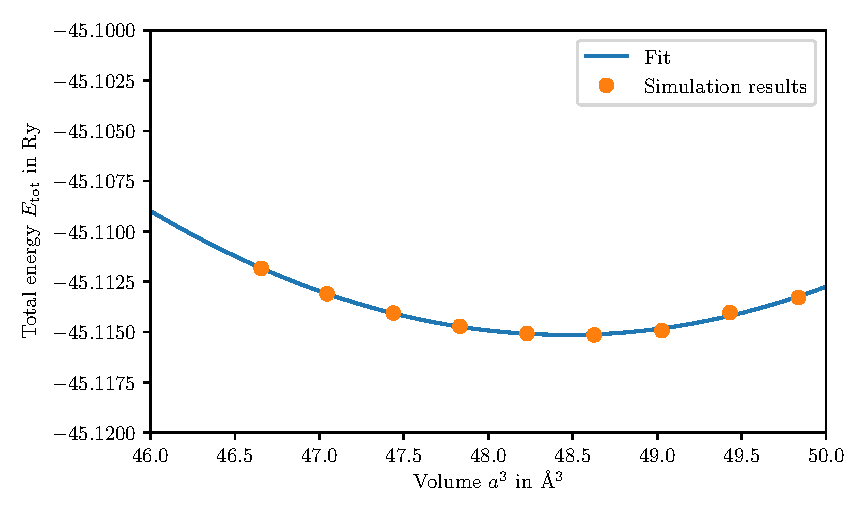
\includegraphics[width=\textwidth]{Figure_lattice_constant_LDA.pdf}
 \caption{Plot of the calculated total energy (using the LDA functional) as a function of the volume of the unit cell. The fit-function which is also shown is a parabola which was fitted to the obtained values in order to determine the equilibrium lattice constant.}
 \label{fig:fig2x}
\end{figure}

\newpage
\subsection{Electronic Structure Calculation}
In order to calculate the projected density of states, we ran a calculation with $4\times 4\times 4=64$ copies of the unit cell.\footnote{Similar to the example provided on the website: https://www.cp2k.org/exercises:2017\_uzh\_cmest:pdos} 
The calculation was performed using PBE and the equilibrium lattice constant which was determined in the previous exercise.
We used the following input file:
\begin{lstlisting}
&GLOBAL
   PROJECT_NAME diamond_PDOS
   RUN_TYPE ENERGY
   PRINT_LEVEL MEDIUM
&END GLOBAL

&FORCE_EVAL
  METHOD QS
  STRESS_TENSOR NONE
  &DFT
      POTENTIAL_FILE_NAME GTH_POTENTIALS
      BASIS_SET_FILE_NAME BASIS_MOLOPT
      &QS
         EPS_DEFAULT 1e-10
         EXTRAPOLATION ASPC
         METHOD GPW
      &END QS
      &MGRID
         NGRIDS 4
         CUTOFF 100
         REL_CUTOFF 60
      &END MGRID
       &SCF
         ADDED_MOS 50
         &DIAGONALIZATION
            ALGORITHM STANDARD
            EPS_ADAPT 0.01
         &END DIAGONALIZATION
         &SMEAR  ON
            METHOD FERMI_DIRAC
            ELECTRONIC_TEMPERATURE [K] 300
         &END SMEAR
         &MIXING
            METHOD BROYDEN_MIXING
            ALPHA 0.2
            BETA 1.5
            NBROYDEN 8
         &END MIXING
      &END SCF
      &XC
          &XC_FUNCTIONAL PBE
          &END XC_FUNCTIONAL
      &END XC
      &PRINT
          &PDOS
              NLUMO -1
              FILENAME ./diamond_pdos
          &END
      &END PRINT
  &END DFT

  &SUBSYS
    &CELL
       A 3.7 0.0000 0.0000
       B 0.00000000 3.7 0.00000
       C 0.00000000 0.000000 3.7
       PERIODIC XYZ
       MULTIPLE_UNIT_CELL 4 4 4
    &END CELL
    &TOPOLOGY
      MULTIPLE_UNIT_CELL 4 4 4
      COORD_FILE_NAME diamond_fd3m.xyz
      COORD_FILE_FORMAT xyz
    &END TOPOLOGY
    &KIND C
       POTENTIAL GTH-PBE
       BASIS_SET DZVP-MOLOPT-SR-GTH
    &END KIND
  &END SUBSYS
&END FORCE_EVAL
\end{lstlisting}
\autoref{fig:fig4} shows a plot of the obtained PDOS for the carbon orbitals. 
\autoref{fig:fig5} shows a PDOS which combines the contributions of all orbitals and was smoothed/smeared by convolving it with a Gaussian.\footnote{This was done using two Python scripts which are provided on the CP2K website: https://wiki.wpi.edu/images/images/b/b7/Pdos.txt and https://wiki.wpi.edu/images/images/4/41/Get-smearing-pdos.txt}
The band gap which makes diamond an insulator is clearly visible.

\begin{figure}[h]
\centering
 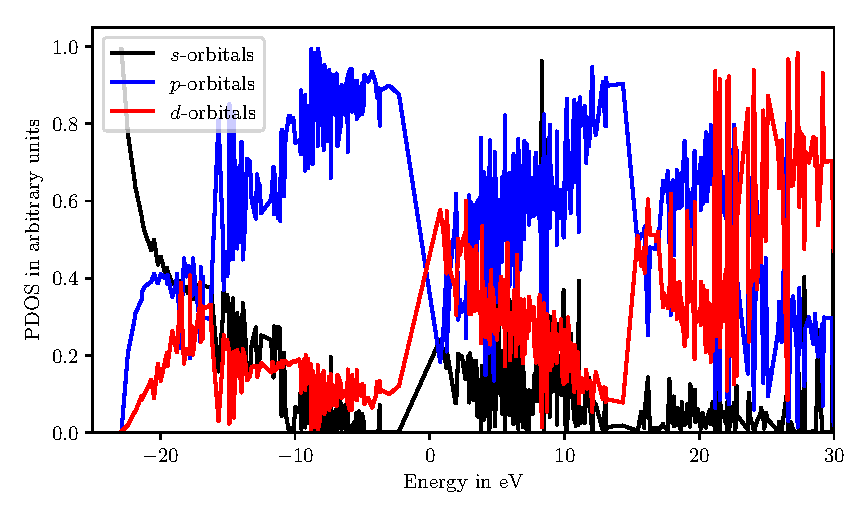
\includegraphics[width=\textwidth]{Figure_PDOS.pdf}
 \caption{PDOS of diamond.}
 \label{fig:fig4}
 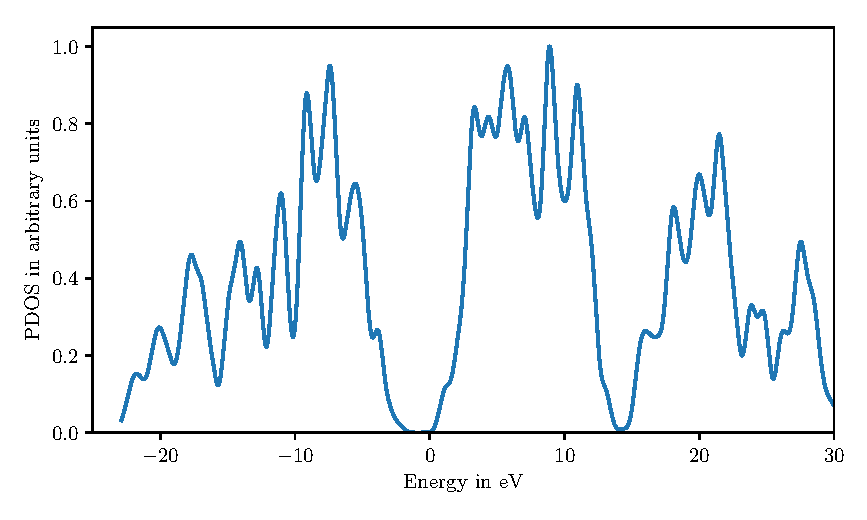
\includegraphics[width=\textwidth]{Figure_smeared_PDOS.pdf}
 \caption{Combined and smeared PDOS of diamond.}
 \label{fig:fig5}
\end{figure}

\end{document}
